\subsubsection{Acrobot}
\begin{figure}[h!]
    \centering
    \scalebox{0.3}{\fbox{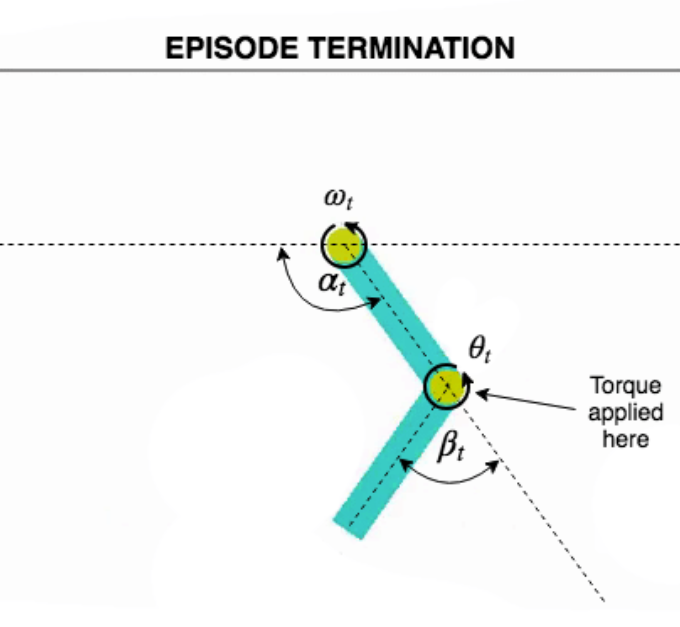
\includegraphics{thesis/images/acrobot_env.png}}}
    \caption{Trò chơi Acrobot}
    \label{fig:flappybird}
\end{figure}
Acrobot là một con lắc 2 liên kết chỉ có khớp thứ hai được kích hoạt. Ban đầu, cả hai liên kết đều hướng xuống dưới. Mục tiêu là để xoay bộ phận đầu cuối ở độ cao mà ít nhất là chiều dài của một liên kết nằm ở phía trên đường cơ sở. Cả hai liên kết có thể xoay tự do và có thể đi qua nhau, tức là, chúng không va chạm khi chúng có cùng một góc. Trò chơi bao gồm các trạng thái của môi trường là các hàm sin() và cos() của 2 khớp góc quay và vận tốc góc khớp đó là [$\cos(\theta_1)$, $\sin(\theta_1)$, $\cos(\theta_2)$, $\sin(\theta_2)$, $\Dot{\theta_1}$, $\Dot{\theta_2}$]. Đối với liên kết đầu tiên, một góc 0 tương ứng với liên kết hướng xuống dưới. Góc của liên kết thứ hai liên quan đến góc của liên kết thứ nhất. Một góc 0 tương ứng với việc có cùng một góc giữa hai liên kết. Trạng thái [1, 0, 1, 0, ..., ...] có nghĩa là cả hai liên kết đều hướng xuống dưới. Các g
hành động cung cấp là áp dụng mô-men +1, 0 hoặc -1 trên khớp nối giữa hai liên kết con lắc. 

Chiều dài của mỗi liên kết được khởi tạo ban đầu gọi là $l_1$, $l_2$, cấu hình mạng ANN được sử dụng để học là (6,8,1). Trong đồ án này sẽ định nghĩa các tác vụ dựa theo sự khác nhau về độ dài của liên kết thứ 2:
\begin{table} [H]
    \begin{center}
    \caption{Danh sách các tác vụ thực nghiệm bài toán Acrobot}
    \scalebox{0.9}{\begin{tabular}{|c|c|c|c|c|c|}
    \hline
    \multirow{1}{*}{\textbf{Tham số}} & \multicolumn{1}{c|}{\textbf{Tác vụ 1}} & \multicolumn{1}{c|}{\textbf{Tác vụ 2}} & \multicolumn{1}{c|}{\textbf{Tác vụ 3}} & \multicolumn{1}{c|}{\textbf{Tác vụ 4}} & \multicolumn{1}{c|}{\textbf{Tác vụ 5}} \\ \hline
    $l_2$ & $l_2=0.8$ & $l_2=0.9$ & $l_2=1.0$ & $l_2=1.1$ & $l_2=1.2$ \\\hline
    \end{tabular}}
    \end{center}
    \label{tab:result:flappybird}
\end{table}

\subsubsection{PixelCopter}
\begin{figure}[h!]
    \centering
    \scalebox{0.5}{\fbox{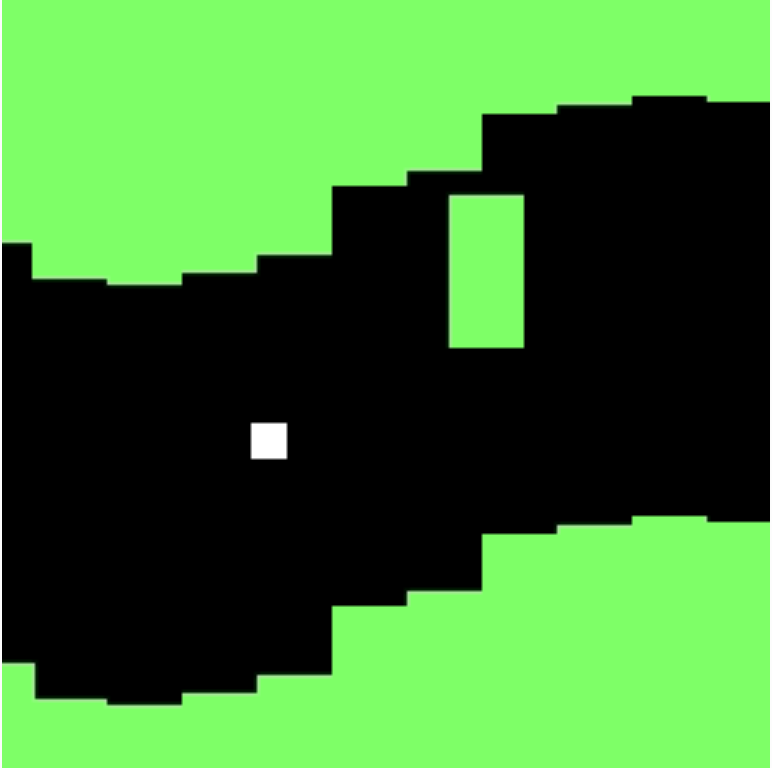
\includegraphics{thesis/images/pixelcopter.png}}}
    \caption{Trò chơi PixelCopter}
    \label{fig:flappybird}
\end{figure}
Pixelcopter là trò chơi đòi hỏi người chơi phải vượt qua các vật cản bên trong một hang động. Đây là bản sao chép của trò chơi máy bay trực thăng nổi tiếng (thuật ngữ gốc: \emph{helicopter}) với người chơi chỉ là một đơn vị pixel khiêm tốn. 
Với mỗi khối đơn vị chiều dài mà người chơi vượt qua sẽ nhận được một điểm thưởng là +1. Khi trò chơi kết thúc sẽ nhận được một điểm thưởng âm là -1. Trò chơi kết thúc khi người choi va đập vào thành hang, hoặc các chướng ngại vật trong hang. Trạng thái của trò chơi được biểu diễn bởi một véc-tơ 7 chiều mô tả vị trí của pixel và các vật cản ở gần. Để mô hình hóa policy của bài toán dưới dạng mạng ANN, đồ án sử dụng một mạng ANN có cấu trúc là (7,8,1) tương ứng với đầu vào, lớp ẩn, đầu ra của policy.

Trong môi trường của trò chơi có một tham số là momentum ảnh hưởng đến tốc độ, và vị trí sau mỗi hành động của pixel. Trong đồ án này sẽ định nghĩa các tác vụ dựa theo sự khác nhau về momentum giữa các môi trường:
\begin{table} [H]
    \begin{center}
    \caption{Danh sách các tác vụ thực nghiệm bài toán Pixelcopter}

    \scalebox{0.85}{\begin{tabular}{|c|c|c|c|c|c|}
    \hline
    \multirow{1}{*}{\textbf{Tham số}} & \multicolumn{1}{c|}{\textbf{Tác vụ 1}} & \multicolumn{1}{c|}{\textbf{Tác vụ 2}} & \multicolumn{1}{c|}{\textbf{Tác vụ 3}} & \multicolumn{1}{c|}{\textbf{Tác vụ 4}} & \multicolumn{1}{c|}{\textbf{Tác vụ 5}} \\ \hline
    momentum & $momentum=0$ & $momentum=0.1$ & $momentum=0.2$ & $momentum=0.3$ & $momentum=0.4$\\\hline
    \end{tabular}}
    \end{center}
    \label{tab:result:flappybird}
\end{table}

\subsubsection{FlappyBird}
\begin{figure}[h!]
    \centering
    \scalebox{0.5}{\fbox{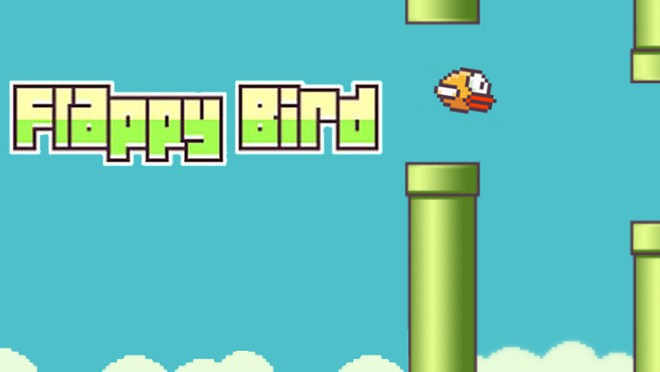
\includegraphics{flappy-bird_tbqj.jpg}}}
    \caption{Trò chơi FlappyBird}
    \label{fig:flappybird}
\end{figure}
Là trò chơi mà ở đó tác nhân (chú chim) phải vượt qua được khoảng trống giữa các ống. Trong trò chơi tác nhân chỉ thực hiện 2 hành động: hướng lên, hướng xuống. Mũi tên hướng lên khiến chim trong trò chơi sẽ đi lên, mũi trên hướng xuống khiến chim đi xuống. Trong trường hợp chim đập xuống đất, đập vào thành ống hoặc đập lên phía trên màn hình thì trò chơi sẽ kết thúc. Mỗi lượt chim qua một ống sẽ được tính là được thêm $+1$ điểm thưởng. Mỗi lần tới trạng thái kết thúc sẽ nhận được một điểm thưởng âm là $-1$. Có 8 trạng thái biểu diễn vị trí 2D của chim, vị trí của vật cản tiếp theo, vị trị của vật cản tiếp theo sau đó. Với bài toán này trong đồ án sẽ sử dụng một mạng ANN có cấu hình là $(8,4,1)$ tương ứng với đầu vào, lớp ẩn, đầu ra của mạng để có thể học được mô hình policy của bài toán.

Trong môi trường của trò chơi có một tham số là trọng lực (thuật ngữ gốc: \emph{gravity}. Trong đồ án này sẽ định nghĩa các tác vụ dựa theo sự khác nhau về trọng lực giữa các môi trường:
\begin{table} [H]
    \begin{center}
    \caption{Danh sách các tác vụ thực nghiệm bài toán FlappyBird}

    \scalebox{0.9}{\begin{tabular}{|c|c|c|c|c|c|}
    \hline
    \multirow{1}{*}{\textbf{Tham số}} & \multicolumn{1}{c|}{\textbf{Tác vụ 1}} & \multicolumn{1}{c|}{\textbf{Tác vụ 2}} & \multicolumn{1}{c|}{\textbf{Tác vụ 3}} & \multicolumn{1}{c|}{\textbf{Tác vụ 4}} & \multicolumn{1}{c|}{\textbf{Tác vụ 5}} \\ \hline
    gravity & $gravity=0.8$ & $gravity=1.8$ & $gravity=2.8$ & $gravity=3.8$ & $gravity=4.8$\\\hline
    \end{tabular}}
    \end{center}
    \label{tab:result:flappybird}
\end{table}
